\section{\acf{DTN}}

\subsection{Introduction}

\begin{frame}
  \frametitle{\acf{BP7}}

  \begin{itemize}
  \item Describes both a \acs{DTN} architecture and protocol
  \item Still in active development
  \item Latest draft was released on 04.08.2019
  \item Aims to obsolete Bundle Protocol Version 6, RFC 5050
  \end{itemize}
\end{frame}

\subsection{Nodes and Endpoints}

\begin{frame}
  \frametitle{Nodes and Endpoints}

  \begin{itemize}
  \item Nodes are identified by an Endpoint ID (URI), e.g., \texttt{dtn:node}
  \item A node might be addressed by multiple Endpoint IDs
  \item An Endpoint ID might represent multiple nodes
  \end{itemize}

  \begin{figure}
    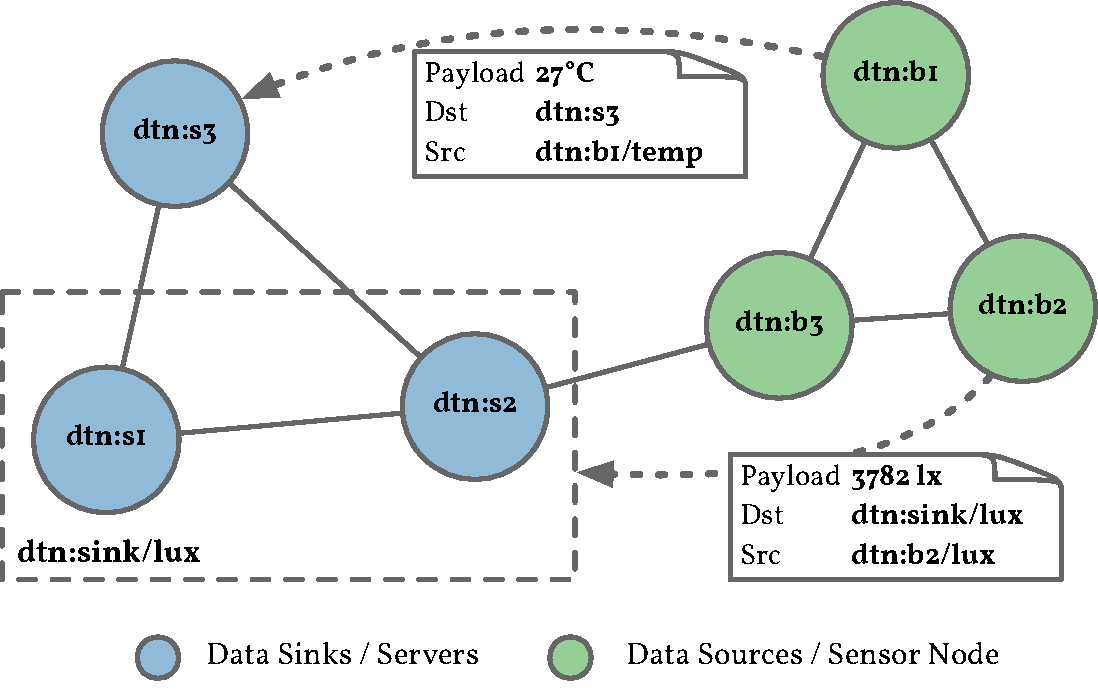
\includegraphics[width=0.6\linewidth,keepaspectratio]{include/nodes-endpoints}
  \end{figure}
\end{frame}

\subsection{Bundles and Blocks}

\begin{frame}
  \frametitle{Bundles and Blocks}

  \begin{itemize}
  \item \acs{BP7} packets are called Bundles
  \item A Bundle is a sequence of Blocks
  \item Binary represented in CBOR, RFC 7049
  \end{itemize}

  \begin{figure}
    \resizebox{\textwidth}{!}{
    \begin{tikzpicture}
    \begin{umlpackage}[fill=white]{Bundle}
      \umlclass[rectangle split parts=2, fill=white, visible on=<1>]{Primary Block}{
        Version: \texttt{7} \\
        Control Flags: \\
          \quad \textit{Status requested for reception} \\
        CRC Type: \textit{CRC32} \\
        Destination EID: \texttt{dtn:sink/lux} \\
        Source node EID: \texttt{dtn:b2/lux} \\
        Report-to EID: \texttt{dtn:b2/lux} \\
        Creation Timestamp: (\texttt{0}, \texttt{23}) \\
        Lifetime: \textit{3600000} \\
        CRC Value: \texttt{67 75 6D 6F}
      }{}
      \umlclass[rectangle split parts=2, visible on=<2>]{Primary Block}{
        Version: \texttt{7} \\
        Control Flags: \\
          \quad \textit{Status requested for reception} \\
        CRC Type: \textit{CRC32} \\
        Destination EID: \texttt{dtn:sink/lux} \\
        Source node EID: \texttt{dtn:b2/lux} \\
        Report-to EID: \texttt{dtn:b2/lux} \\
        Creation Timestamp: (\texttt{0}, \texttt{23}) \\
        Lifetime: \textit{3600000} \\
        CRC Value: \texttt{67 75 6D 6F}
      }{}
      \umlclass[rectangle split parts=2, fill=white, visible on=<3->]{Primary Block}{
        Version: \texttt{7} \\
        Control Flags: \\
          \quad \textit{Status requested for reception} \\
        CRC Type: \textit{CRC32} \\
        Destination EID: \texttt{dtn:sink/lux} \\
        Source node EID: \texttt{dtn:b2/lux} \\
        Report-to EID: \texttt{dtn:b2/lux} \\
        Creation Timestamp: (\texttt{0}, \texttt{23}) \\
        Lifetime: \textit{3600000} \\
        CRC Value: \texttt{67 75 6D 6F}
      }{}
      \umlclass[rectangle split parts=2, fill=white, x=4.75, y=1.054, visible on=<-2>]{Hop Count Block}{
        Type Code: \texttt{9} \\
        Number: \texttt{2} \\
        Control Flags: \textit{None} \\
        CRC Type: \textit{None} \\
        Data: (\texttt{64}, \texttt{42})
      }{}
      \umlclass[rectangle split parts=2, fill=white, x=8.6, y=1.054, visible on=<-2>]{Payload Block}{
        Type Code: \texttt{1} \\
        Number: \texttt{1} \\
        Control Flags: \textit{None} \\
        CRC Type: \textit{None} \\
        Data: \texttt{0E C6}
      }{}
      \umlclass[rectangle split parts=2, x=4.75, y=1.054, visible on=<3>]{Hop Count Block}{
        Type Code: \texttt{9} \\
        Number: \texttt{2} \\
        Control Flags: \textit{None} \\
        CRC Type: \textit{None} \\
        Data: (\texttt{64}, \texttt{42})
      }{}
      \umlclass[rectangle split parts=2, fill=white, x=4.75, y=1.054, visible on=<4>]{Hop Count Block}{
        Type Code: \texttt{9} \\
        Number: \texttt{2} \\
        Control Flags: \textit{None} \\
        CRC Type: \textit{None} \\
        Data: (\texttt{64}, \texttt{42})
      }{}
      \umlclass[rectangle split parts=2, x=8.6, y=1.054, visible on=<3->]{Payload Block}{
        Type Code: \texttt{1} \\
        Number: \texttt{1} \\
        Control Flags: \textit{None} \\
        CRC Type: \textit{None} \\
        Data: \texttt{0E C6}
      }{}
      \draw[decorate,decoration={brace,amplitude=10pt},xshift=-4pt,visible on=<3>]
        (10.5,-0.75) -- (3.1,-0.75) node [black,midway,yshift=-20pt]{Canonical Blocks};
    \end{umlpackage}
    \end{tikzpicture}
    }
  \end{figure}
\end{frame}
